%%%%%%%%%%%%%%%%%%%%%%%%%%%%%%%%%%%%%%%%%%%%%%%%%%%%%%%%%%%%%%%%%%%%%%%%%%%%%%%%%%%%%%
% Grundlagen                
%%%%%%%%%%%%%%%%%%%%%%%%%%%%%%%%%%%%%%%%%%%%%%%%%%%%%%%%%%%%%%%%%%%%%%%%%%%%%%%%%%%%%%
\section{Grundlagen Digitaltechnik II}

1975: "The Moore's Low"(Gorden E. Moore, Inter Co-Founder): Anzahl Transistoren auf 1 Chip verdoppelt sich alle 2 Jahre\\

\begin{minipage}{0.5\textwidth}
	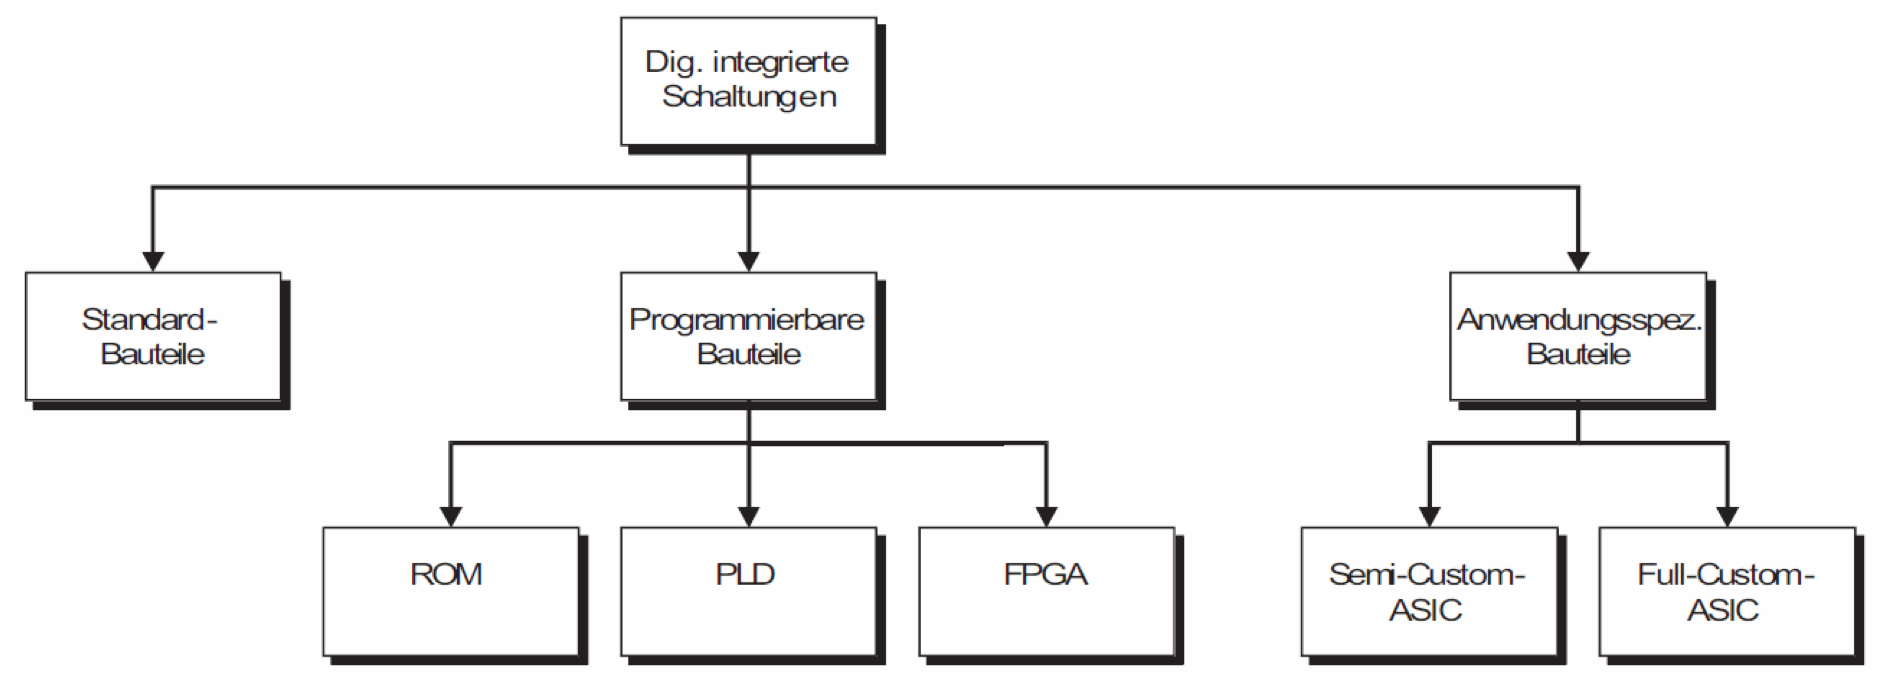
\includegraphics[width=\textwidth]{./bilder/Klassierung}
\end{minipage}
\begin{minipage}[b]{0.5\textwidth}
	\begin{tabular}{l l l}
		SDT-Bauteile 		& Digitale Gates						& AND, OR, ...\\
							& Flipflops 							& \\
		\hline
		Programmier-	 	& ROM {\tiny Read Only Memory}			& PROM {\tiny(one time programmable)}\\
		bare				&										& EPROM {\tiny(eresable with UV)} \\
							&										& EEPROM {\tiny(eresabel with Voltage)}\\
							&										& FLASCH {\tiny (Spezielle EEPROMs)}\\
							\cline{2-3}
							& PDL {\tiny Programable Logic Device}	& PAL {\tiny Programmable Array Logic}\\
							& 										& GAL {\tiny Generic Array Logic} \\
							&										& CPLD {\tiny Complex CLD} \\
							\cline{2-3}
	\end{tabular}
\end{minipage}

\begin{tabular}{l l l l}
	Programmierbare	 		& FPGA {\tiny Field Programmable Gate Array}	& \multicolumn{2}{l}{Im Gegensatz zu PLDs hat es eine regelmässige Strucktur, die in Logik-}\\
	\multicolumn{2}{c}{\multirow{10}{*}{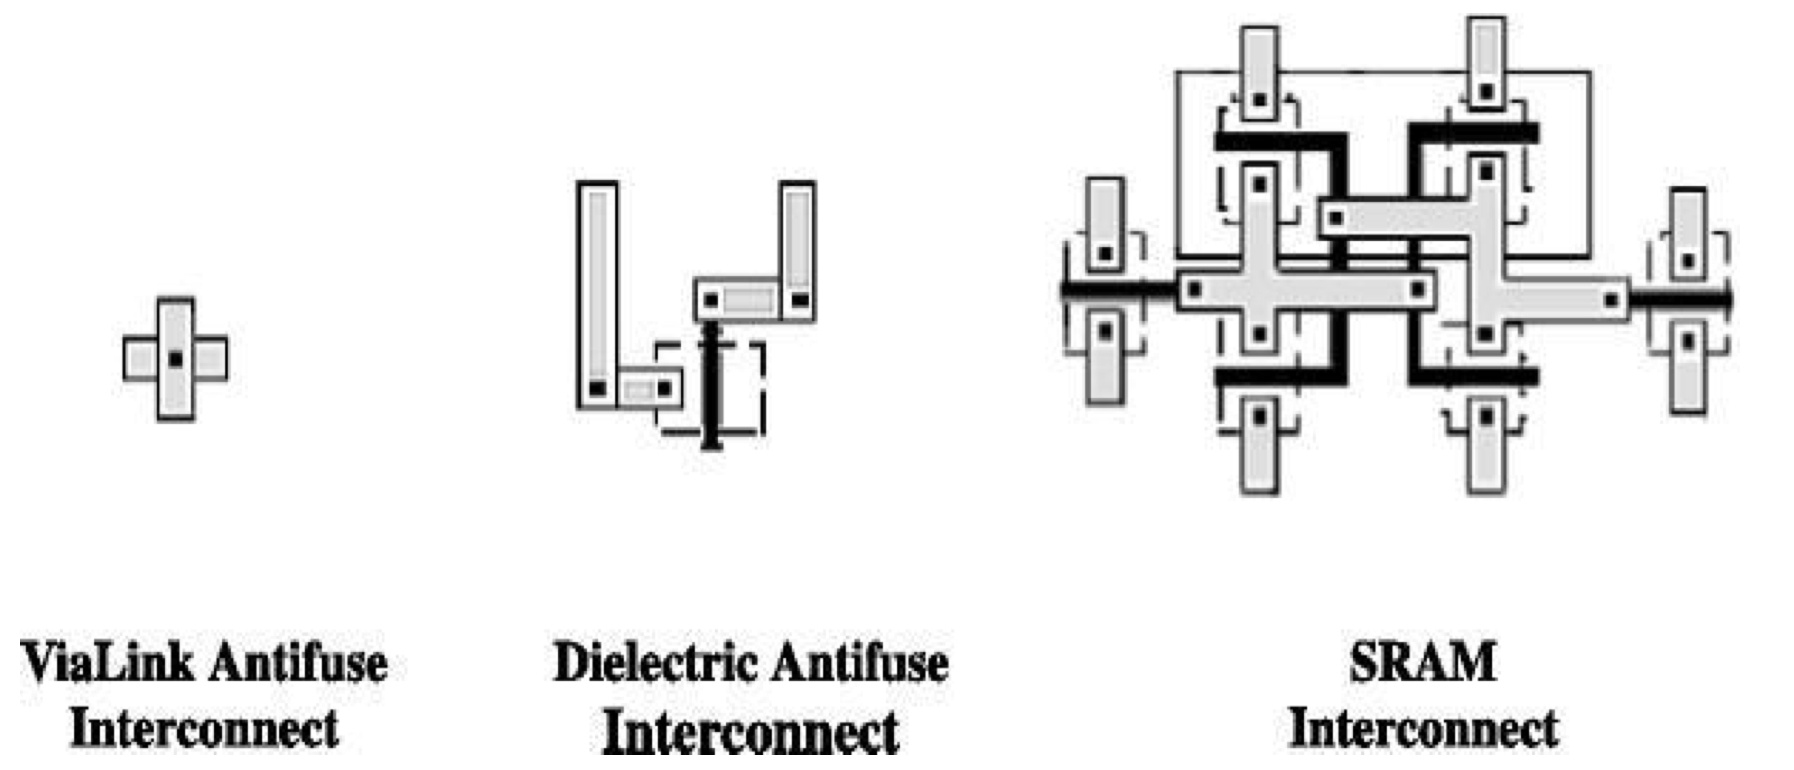
\includegraphics[width=180pt]{./bilder/SRAM}}}	&\multicolumn{2}{l}{ (bei Xilinx CBL) und I/O Blöcke (bei Xilinx IOB)}\\
							&												& \multicolumn{2}{l}{ Man kann Pullup- und Pulldouwnwiderstände hinzuschalten }\\
							&												& \multicolumn{2}{l}{ Schaltpegel sind TTL und CMOS kompatibel}\\
							&		& SRAM - Zelle 							& \multicolumn{1}{|l}{ Antifuse - Technologie}\\
							\cline{3-4}
							&		& Mehrfach Programmierbar				& \multicolumn{1}{|l}{ Verbindung durch Durch-}\\
							&		& Löscht wenn Speisung unterbrochen		& \multicolumn{1}{|l}{ schweissen der Isolation}\\
							&		& hohe Kapazität {\tiny unprogrammiert}	& \multicolumn{1}{|l}{ viel kleiner als SRAM}\\
							&		& geringer Leitwert {\tiny programmiert}& \multicolumn{1}{|l}{ nicht wiederverwendbar}\\
							&		& Stärker verbreitet	 				& \multicolumn{1}{|l}{ sicherer als SRAM}\\
							&		& kann kleine Daten Speichern			& \multicolumn{1}{|l}{ $\rightarrow$ Einsatz im Weltraum}\\
							&		& Startprogramm(e) oft auf PROMS		& \multicolumn{1}{|l}{ }\\
	\hline
	Anwendungsspeziefische	& Semi-Costom									& \multicolumn{2}{l}{Vorgegebenes Grunddesign$\rightarrow$Nutzer macht nur noch Netzmaske}\\
							& 												& \multicolumn{2}{l}{billiger da in Grossen Mengen produziert}\\
							& 												& \multicolumn{2}{l}{kann selten optimal ausgenutzt werden}\\
							\cline{2-4}
							& Full-Custom									& \multicolumn{2}{l}{Spezifische Schaltungen $\rightarrow$ Spezialanfertigung $\rightarrow$ hohe Kosten}\\
							& 												& \multicolumn{2}{l}{Nur in Grossen Mengen rentabel}\\
							& 												& \multicolumn{2}{l}{kann selten optimal ausgenutzt werden}\\
\end{tabular}

